\renewcommand\refname{Literaturverzeichnis}
\addcontentsline{toc}{section}{Literaturverzeichnis}
\printbibliography
\cleardoublepage
\listoffigures


\clearpage

\appendix

\section{Aufgabenstellung}
\begin{figure}[h]
    \centering
    \begin{minipage}[b]{0.8\textwidth}
        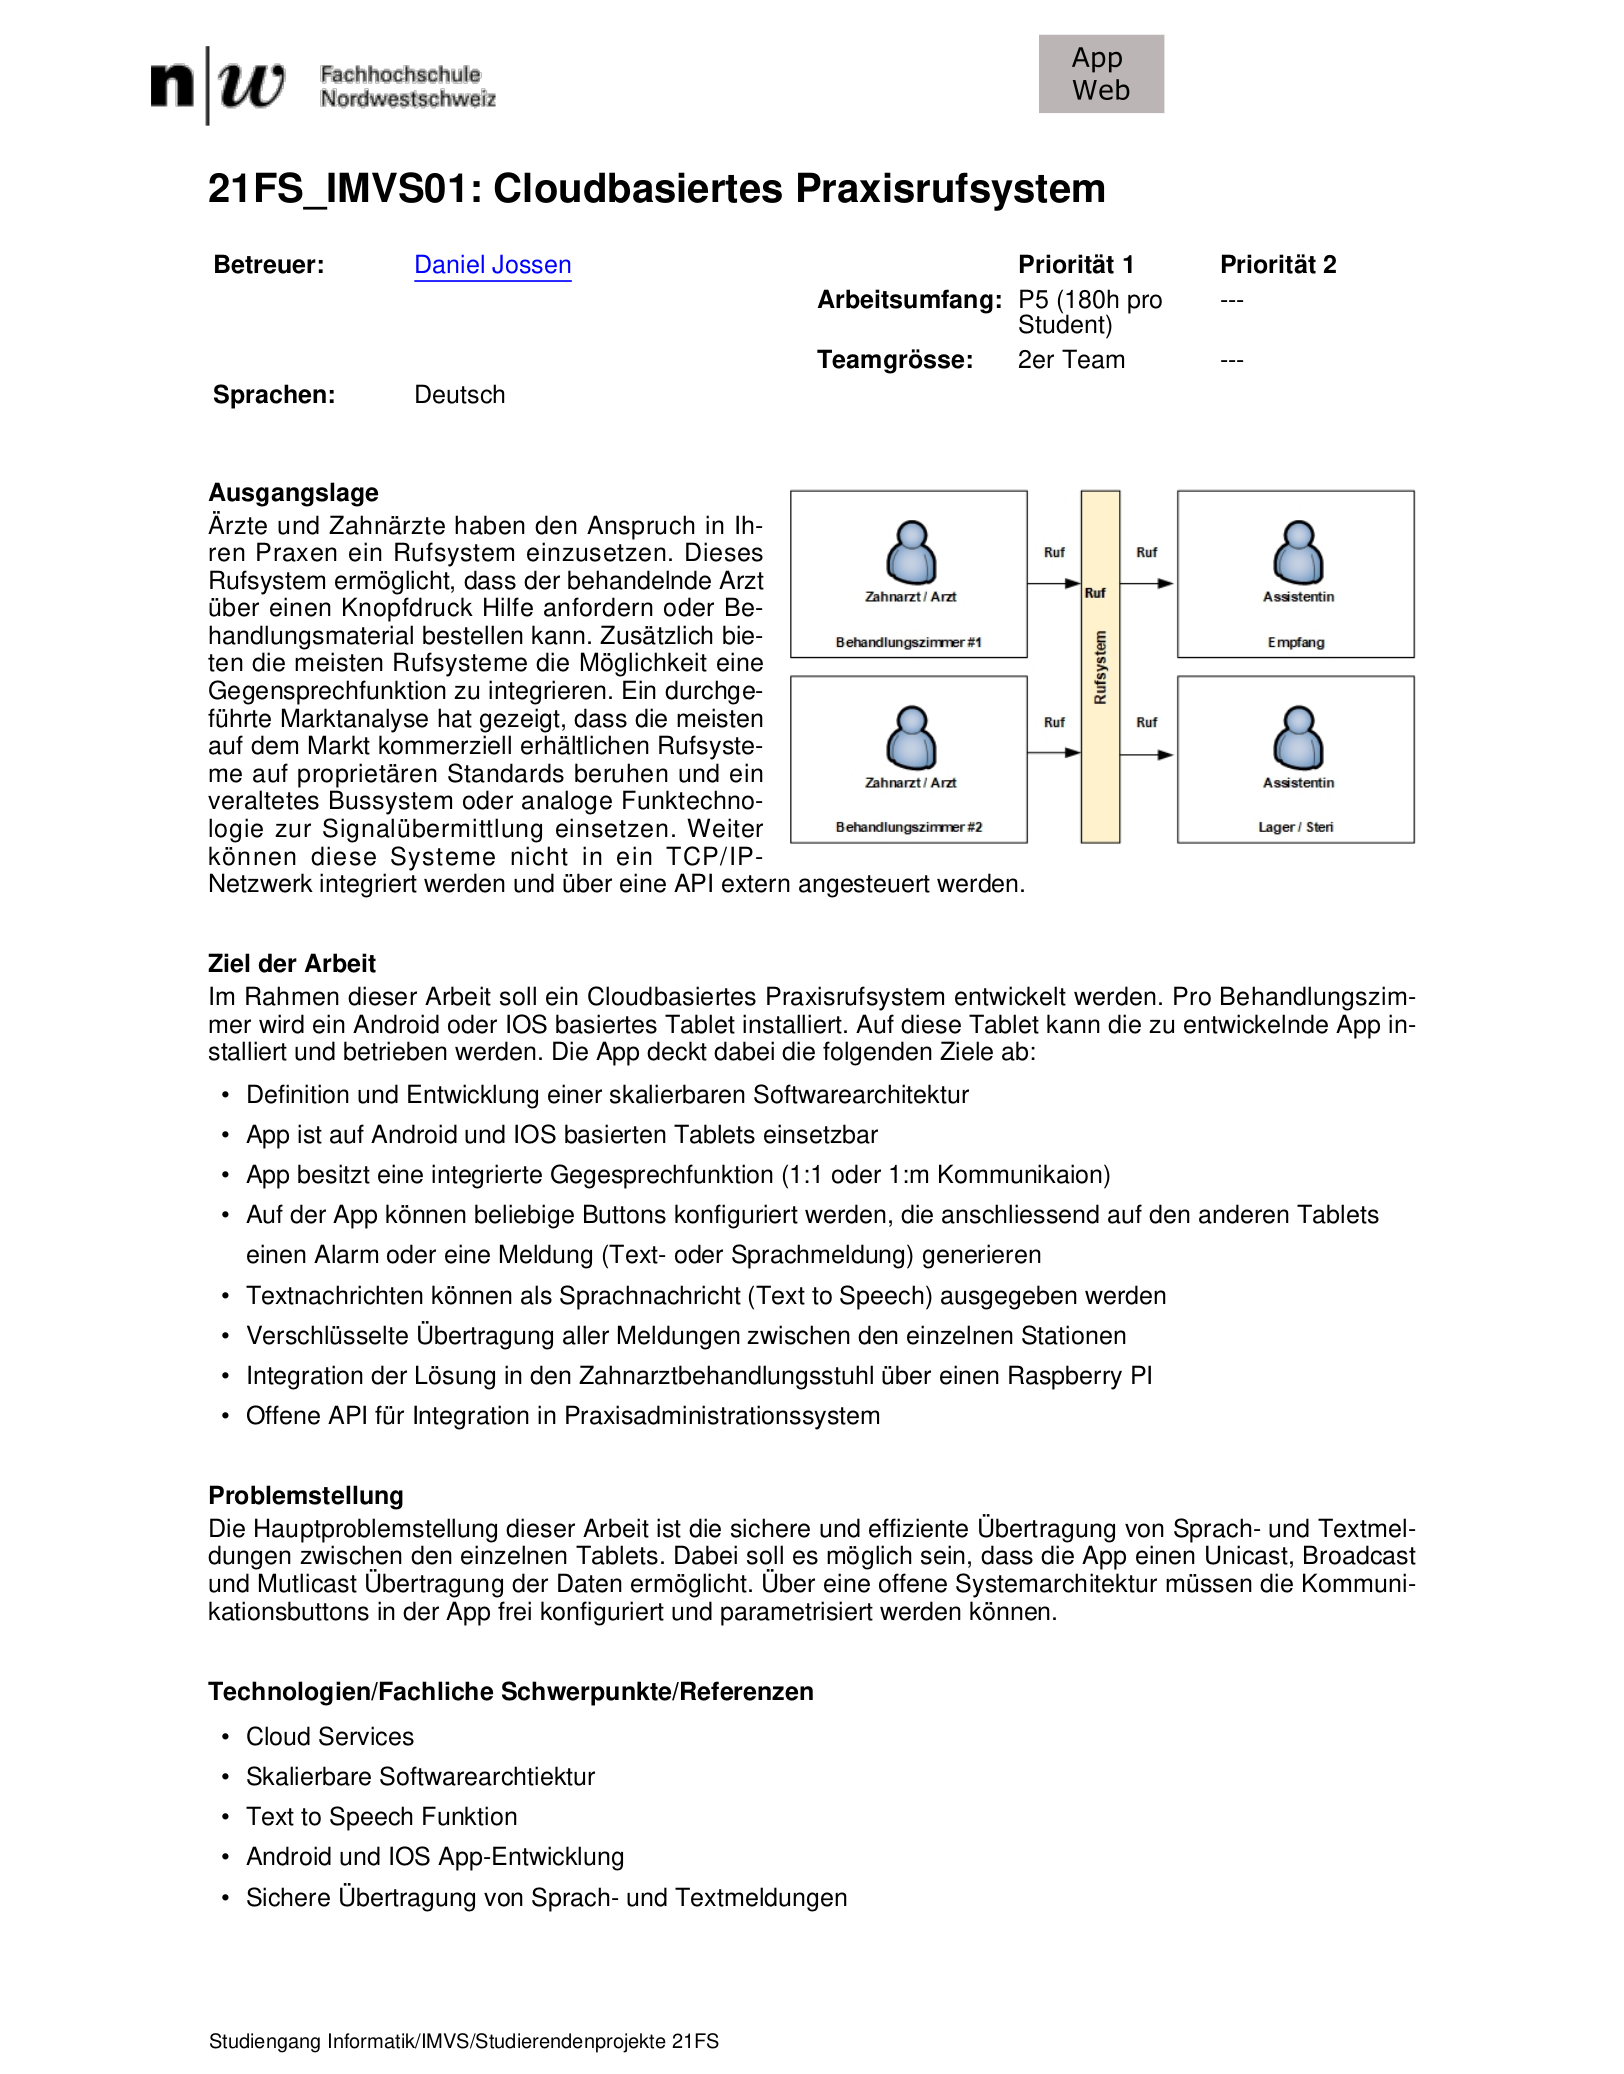
\includegraphics[width=\textwidth]{graphics/aufgabenstellung}
        \caption{Aufgabenstellung}
    \end{minipage}
\end{figure}

\clearpage


\section{Quellcodeverwaltung}

Sämtlicher Quellcode der im Rahmen des Projektes entsteht, wurde mit Git verwaltet. Der Quellcode ist für Berechtigte unter dem Projekt IP5-Cloudbasiertes-Praxisrufsystem auf github.com einsehbar.
(Referenz https://github.com/IP5-Cloudbasiertes-Praxisrufsystem). Berechtigungen können bei Joshua Villing oder Kevin Zellweger angefordert werden.


\section{Benutzerhandbuch}

\subsubsection*{Mobile Client}

\textbf{Anmeldung und Konfiguration}

\begin{enumerate}
    \item Mobile Client Applikation öffnen
    \item Anmeldedaten eingeben und bestätigen
    \item Gewünschte Konfiguration auswählen
\end{enumerate}

\textbf{Benachrichtigung empfangen}

\begin{enumerate}
    \item In Mobile Client anmelden.
    \item In Navigationsleiste (unten) "Home" auswählen.
    \item Button mit dem gewünschten Titel antippen.
    \item Die Benachrichtigung wird automatisch versendet.
\end{enumerate}

\textbf{Benachrichtigung Auflisten und Quittieren}

\begin{enumerate}
    \item In Mobile Client anmelden.
    \item In Navigationsleiste (unten) "Inbox" auswählen.
    \item In dieser Ansicht sehen Sie alle empfangenen noch nicht quittierten Benachrichtigungen.
    \item Zum Quittieren einer Benachrichtigung kann diese angetippt werden.
\end{enumerate}

\textbf{Abmeldung}

\begin{enumerate}
    \item Mobile Client Applikation öffnen
    \item Auf den Namen in der Kopfleiste tippen
    \item Logout bestätigen
\end{enumerate}

\subsubsection*{Admin UI}

\textbf{Anmeldung}

\begin{enumerate}
    \item Admin UI im Browser öffnen
    \item Anmeldedaten eingeben und bestätigen. Die Anmeldedaten erhalten Sie nach Installation des Systems vom Betreiber.
\end{enumerate}

\textbf{Einträge hinzufügen}
\begin{enumerate}
    \item Melden Sie sich im Admin UI an.
    \item Wählen Sie auf der Linken Seite die Kategorie die Sie verwalten möchten.
    \item Auf dieser Seite können Sie nun Einträge zur gewählten Kategorie verwalten:
    \begin{itemize}
        \item Klicken Sie oben rechts auf die Schaltfläche "Create" um einen neuen Eintrag zu erstellen.
        \item Klicken Sie auf einen Eintrag in der Liste um ihn zu bearbeiten.
        \item Klicken Sie die Checkbox auf der Linken Seite eines Eintrages und dann auf die Schaltfläche "löschen" um einen Eintrag zu löschen.
    \end{itemize}
\end{enumerate}

\textbf{Praxisruf konfigurieren}
\begin{enumerate}
    \item Melden Sie sich im Admin UI an.
    \item Erfassen Sie in der Kategorie "User" pro Praxiszimmer einen Benutzer.
    \item Erfassen Sie in der Kategorie "Client" pro Gerät und Zimmer einen Eintrag und weisen Sie ihn dem Benutzer des entsprechenden Zimmers zu.
    \item Erfassen Sie in der Kategorie "Notification Types" alle Benachrichtigungen die Sie zur Verfügung stellen möchten.
    \item Erfassen Sie in der Kategorie "Configurations" pro Gerät und Zimmer einen Eintrag und weisen es dem entsprechenden Client zu.
    \item Unter Notification Types können die Benachrichtigungen auswählen, die auf diesem Gerät zum Versenden verfügbar sind.
    \item Unter Rule Parameters können Sie Regeln definieren, welche Benachrichtigungen diesem Client zugestellt werden.
\end{enumerate}


\section{Installationsanleitung}

\subsubsection*{Mobile Client}
\textbf{TODO}
?? Cloud Service url configuration \\
?? FCM Integration configuration \\

\subsubsection*{Admin UI}
\begin{enumerate}
    \item Setup Amplify
    \item Setup Domain
\end{enumerate}

\subsubsection*{Cloud Service}

\begin{enumerate}
    \item Setup FCM
    \item Setup Beanstalk
    \item Pipeline
    \item Setupt RDS
    \item Setup Domain
    \item Setup EB
    \item Configure Environment
    \item Create administrator
\end{enumerate}

\clearpage

\section{Features und Testszenarien}

\subsubsection*{F01 - Benachrichtigungen Versenden}
\begin{tabbing}
    Left \= Middle \= Right \= Right \kill
    Scenario S01: \> \> \> Benachrichtigung versenden\\ \\
    Given:  \> \> \> Benutzer ist vollständig angemeldet\\
    And: \>    \> \> Mindestens ein Empfänger ist konfiguriert\\
    When:   \> \> \> Praxismitarbeiter tippt auf einen Benachrichtigungs-Button\\
    Then:   \> \> \> Benachrichtigung wird an den zentralen Cloud Service gesendet\\
    And: \>    \> \> Benachrichtigung wird an alle Mobile Clients versendet\\
    \> \>  \> die sich für diese Benachrichtigung subscribed haben weitergeleitet\\
    And:   \> \> \> Praxismitarbeiter erhält optische Rückmeldung, dass Benachrichtigung versendet wurde\\

    \\
    Scenario S02: \>  \> \> Keine Empfänger konfiguriert\\ \\
    Given:  \> \> \> Benutzer ist vollständig angemeldet\\
    And:  \> \>   \> Kein Empfänger ist konfiguriert\\
    When:  \> \>  \> Praxismitarbeiter tippt auf einen Benachrichtigungs-Button\\
    Then:  \> \>  \> Benachrichtigung wird an den zentralen Cloud Service gesendet\\
    And:  \> \>   \> Benachrichtigung wird nicht weitergeleitet\\

\end{tabbing}


\subsubsection*{F02 - Benachrichtigungen Empfangen}
\begin{tabbing}
    Left \= Middle \= Right \= Right  \kill

    Scenario S03: \>  \> \> Empfangen\\ \\
    Given: \>  \> \>  Eine Benachrichtigung wurde von Mobile Client versendet\\
    When: \>  \> \>   Cloud Service Notification an Empfänger Mobile Client weiterleitet\\
    Then: \>  \> \>   Wird die Benachrichtigung vom Empfänger Mobile Client empfangen\\
    And: \>  \> \>    In einer Übersicht für empfangene Benachrichtigung angezeigt.\\

\end{tabbing}

\clearpage
\subsubsection*{F03 - Fehlgeschlagene Benachrichtigungen}

\begin{tabbing}
    Left \= Middle \= Right \= Right  \kill
    Scenario S04: \> \> \>  Fehler Rückmeldung\\ \\
    Given: \> \> \>   Eine Benachrichtigung wurde von Mobile Client versendet\\
    When: \> \> \>    Weiterleitung von Cloud Service Notification an Empfänger schlägt auf Service Seite fehl\\
    Then: \> \> \>    Der Praxismitarbeiter wird über den Fehler informiert\\
    And: \> \> \>     Der Praxismitarbeiter hat die Möglichkeit die fehlgeschlagenen Benachrichtigungen zu wiederholen\\
    \\
    Scenario S05: \> \> \>  Confirm Retry\\ \\
    Given: \> \> \>   Benachrichtigung ist fehlgeschlagen\\
    And: \> \> \>     Dialog zum Wiederholen wird angezeigt\\
    When: \> \> \>    Praxismitarbeiter bestätigt, dass wiederholt werden soll\\
    Then: \> \> \>    Der Cloudservice versucht erneut, die fehlgeschlagenen zuzustellen\\
    \\
    Scenario S06: \> \> \>  Cancel Retry\\ \\
    Given: \> \> \>   Benachrichtigung ist fehlgeschlagen\\
    And: \> \> \>     Dialog zum Wiederholen wird angezeigt\\
    When: \> \> \>    Praxismitarbeiter klick, dass nicht wiederholt werden soll\\
    Then: \> \> \>    Werden die fehlgeschlagenen nicht wiederholt\\
    And: \> \> \>     Zurück zur Notificationsansicht\\

\end{tabbing}

\subsubsection*{F04 - Über Benachrichtigungen Notifizieren}
\begin{tabbing}
    Left \= Middle \= Right \= Right  \kill
    Scenario S07: \> \> \>  Foreground\\ \\
    Given: \> \> \>   Mobile Client ist geöffnet\\
    When: \> \> \>    Eine Benachrichtigung wird vom Mobile Client empfangen\\
    Then: \> \> \>    Ein Audio Signal erklingt\\
    \\
    Scenario S08: \> \> \>  Background\\ \\
    Given: \> \> \>   Mobile Client läuft im Hintergrund\\
    When: \> \> \>    Eine Benachrichtigung wird vom Mobile Client empfangen\\
    Then: \> \> \>    Ein Audio Signal erklingt\\
    And: \> \> \>     Eine Push-Benachrichtigung wird angezeigt\\
    \\
    Scenario S09: \> \> \>  Nicht Quittiert\\ \\
    Given: \> \> \>   Mobile Client ist geöffnet\\
    And: \> \> \>     Eine Benachrichtigung wurde empfangen\\
    When: \> \> \>    Benachrichtigung wird nicht quittiert\\
    Then: \> \> \>    Ein Audio Signal erklingt\\
    And: \> \> \>     Das Audio Signal wiederholt sich alle 30 Sekunden, bis die Benachrichtigung quittiert wurde.\\
\end{tabbing}

\clearpage

\subsubsection*{F05 - Login Mobile Client}
\begin{tabbing}
    Left \= Middle \= Right \= Right  \kill
    Scenario S10: \> \> \>  Startbildschirm, wenn nicht angemeldet\\ \\
    Given: \> \> \>   Mobile Client is geöffnet\\
    When: \> \> \>  Benutzer ist nicht angemeldet\\
    Then: \> \> \>  Benutzer wird zum Login aufgefordert\\
    \\
    Scenario S11: \> \> \>  Startbildschirm, wenn angemeldet\\ \\
    Given: \> \> \>   Mobile Client is geöffnet\\
    When: \> \> \>  Benutzer ist angemeldet\\
    Then: \> \> \>  Konfiguration, die der Benutzer zuletzt gewählt hat, wird angezeigt\\
    And: \> \> \>    Benachrichtigungs-Buttons gemäss Konfiguration werden angezeigt.\\
    \\
    Scenario S12: \> \> \>  Anmelden korrekt\\ \\
    Given: \> \> \>  Benutzer ist nicht angemeldet\\
    And: \> \> \>    Login Screen wird angezeigt\\
    And: \> \> \>     Für den Benutzer sind gültige Konfigurationen erfasst\\
    When: \> \> \>   Benutzer meldet sich mit korrekten Daten an\\
    Then: \> \> \>   Benutzer wird auf nächste Seite geleitet und kann dort die Konfiguration auswählen, die er Benutzen möchte.\\
    \\
    Scenario S13: \> \> \>  Anmelden falsch\\ \\
    Given: \> \> \>  Benutzer ist nicht angemeldet\\
    And: \> \> \>    Login Screen wird angezeigt\\
    When: \> \> \>   Benutzer meldet sich mit falschen Daten an\\
    Then: \> \> \>   Fehlermeldung\\
    And: \> \> \>  Benutzer wird nicht weitergeleitet\\
    \\
    Scenario S14: \> \> \>  Konfiguration Wählen\\ \\
    Given: \> \> \>  Benutzer hat sich korrekt angemeldet\\
    And: \> \> \>    Konfiguration Auswählen Screen wird angezeigt\\
    When: \> \> \>   Der Benutzer wählt die gewünschte Konfiguration\\
    Then: \> \> \>   Der Benutzer wird weitergeleitet\\
    And: \> \> \>    Die gewählte Konfiguration wird geladen\\
    And: \> \> \>    Benachrichtigungs Buttons gemäss Konfiguration werden angezeigt.\\ \\

    Scenario S15: \>  \> \> Logout\\ \\
    Given: \> \> \>  Benutzer ist angemeldet\\
    When: \> \> \>   Benutzer klickt logout\\
    Then: \> \> \>  Benutzer wird zur Login Seite weitergeleitet\\
\end{tabbing}

\clearpage

\subsubsection*{F06 - Konfigurationsverwaltung}
\begin{tabbing}
    Left \= Middle \= Right \= Right  \kill
    Scenario S16: \> \> \>  Login\\ \\
    Given: \> \> \>  Benutzer ist nicht angemeldet\\
    And: \> \> \>    Admin UI Login Screen wird angezeigt\\
    When: \> \> \>   Admin meldet sich mit korrekten Daten an\\
    Then: \> \> \>   Admin wird auf Übersichtsseite weitergeleitet\\ \\

    Scenario S17: \> \> \>  Anmelden falsch\\ \\
    Given: \> \> \>  Benutzer ist nicht angemeldet\\
    And: \> \> \>    Admin UI Login Screen wird angezeigt\\
    When: \> \> \>   Admin meldet sich mit falschen Daten an\\
    Then: \> \> \>   Fehlermeldung wird angezeigt\\
    And: \> \> \>   Admin wird nicht weitergeleitet.\\ \\

    Scenario S18: \> \> \>  Konfiguration verwalten \\ \\
    Given: \> \> \>  Admin ist angemeldet\\
    When: \> \> \>  Admin UI wird aufgerufen\\
    Then: \> \> \>  Alle existierenden Konfigurationen werden angezeigt\\
    And: \> \> \>  Neue Konfigurationen können erstellt werden\\
    And: \> \> \>  Bestehende Konfigurationen können verändert werden\\
    And: \> \> \>  Bestehende Konfigurationen können gelöscht werden\\
\end{tabbing}

\subsubsection*{F07 - Integration Behandlungsstuhl}

Dieses Feature fällt ausserhalb des Projekt Scopes. Dementsprechend wurden dafür noch keine Szenarien definiert.

\subsubsection*{F08 - Text To Speech}
Dieses Feature fällt ausserhalb des Projekt Scopes. Dementsprechend wurden dafür noch keine Szenarien definiert.

\subsubsection*{F09 - Direkte Anrufe}
Dieses Feature fällt ausserhalb des Projekt Scopes. Dementsprechend wurden dafür noch keine Szenarien definiert.

\subsubsection*{F10 - Gruppen Anrufe}
Dieses Feature fällt ausserhalb des Projekt Scopes. Dementsprechend wurden dafür noch keine Szenarien definiert.

\clearpage


\section{Ehrlichkeitserklärung}

«Hiermit erkläre ich, die vorliegende Projektarbeit IP5 - Cloudbasiertes Praxisrufsystem selbständig und nur unter Benutzung der angegebenen Quellen verfasst zu haben.
Die wörtlich oder inhaltlich aus den aufgeführten Quellen entnommenen Stellen sind in der Arbeit als Zitat bzw. Paraphrase kenntlich gemacht.
Diese Projektarbeit ist noch nicht veröffentlicht worden.
Sie ist somit weder anderen Interessierten zugänglich gemacht noch einer anderen Prüfungsbehörde vorgelegt worden.»

\begin{tabbing}
    \\
    \\
    \\
    Left \= Middle \=  \= Right \kill
    Name \> \> \>    Joshua Villing\\
    Ort \> \> \>    Aarau \\
    Datum \> \> \>    19.08.2021\\
    \\
    Unterschrift \> \> \>     ............................\\
    \\
    \\
    Left \= Middle \= Right \kill
    Name \> \> \>    Kevin Zellweger\\
    Ort \> \>\>    Aarau\\
    Datum \> \> \>    19.08.2021\\
    \\
    Unterschrift \> \> \>    ............................\\
\end{tabbing}
